\chapter{Drone Hardware}
\label{ch:drone}

The drone used at the time of writing this thesis is a Snapdragon drone with a Pixhawk flight controller and a VOXL2 embedded processor. \cref{fig:appendix_drone_hardware} shows an image of this rotorcraft hardware. On this drone setup there is a tracking camera and a stereo camera. Note that the landing supports of the drone are significantly farther apart than for the model in the simulation. This is why the simulated stereo camera in Gazebo had to be placed further away from the drone while in reality it was mounted normally on the drone's body.

\begin{figure}[h]
\centering
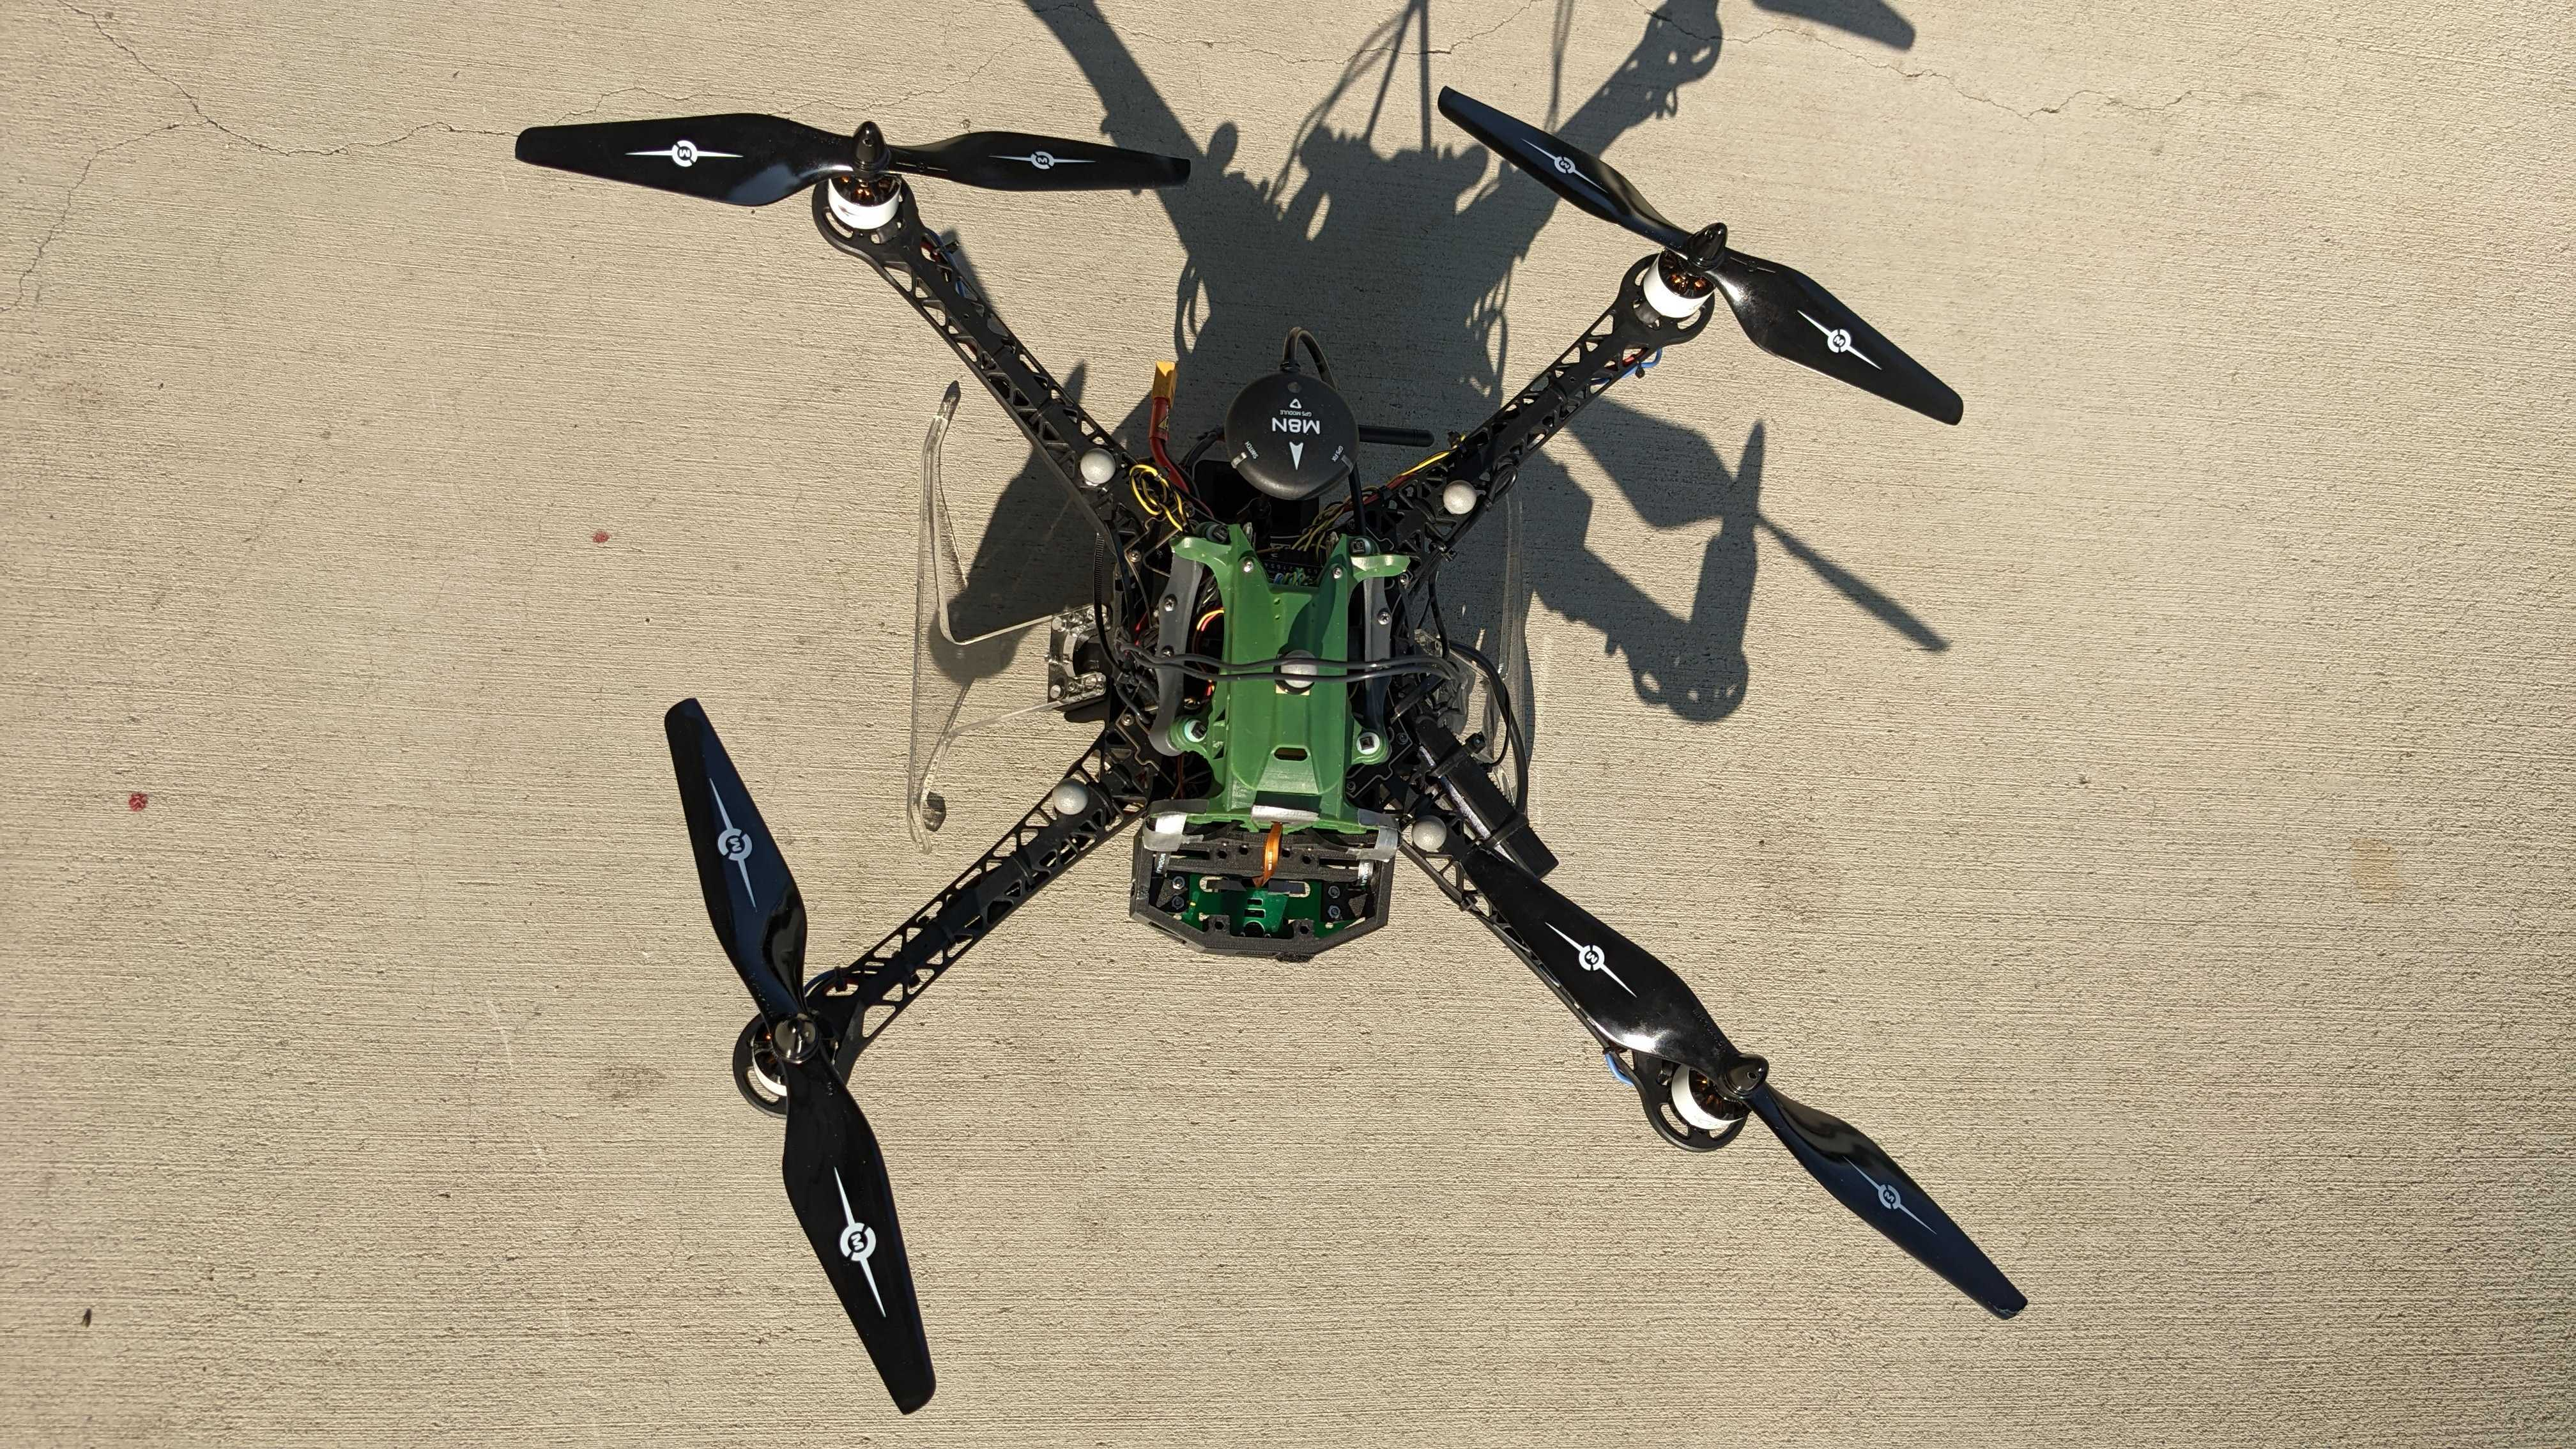
\includegraphics[scale=0.085]{images/appendix/Drone/drone.jpg}
\caption{Snapdragon drone setup}
\label{fig:appendix_drone_hardware}
\end{figure}

\cref{fig:appendix_stereo_camera_hardware} shows the stereo camera according to which the simulation model was implemented.

\begin{figure}[h]
    \centering
    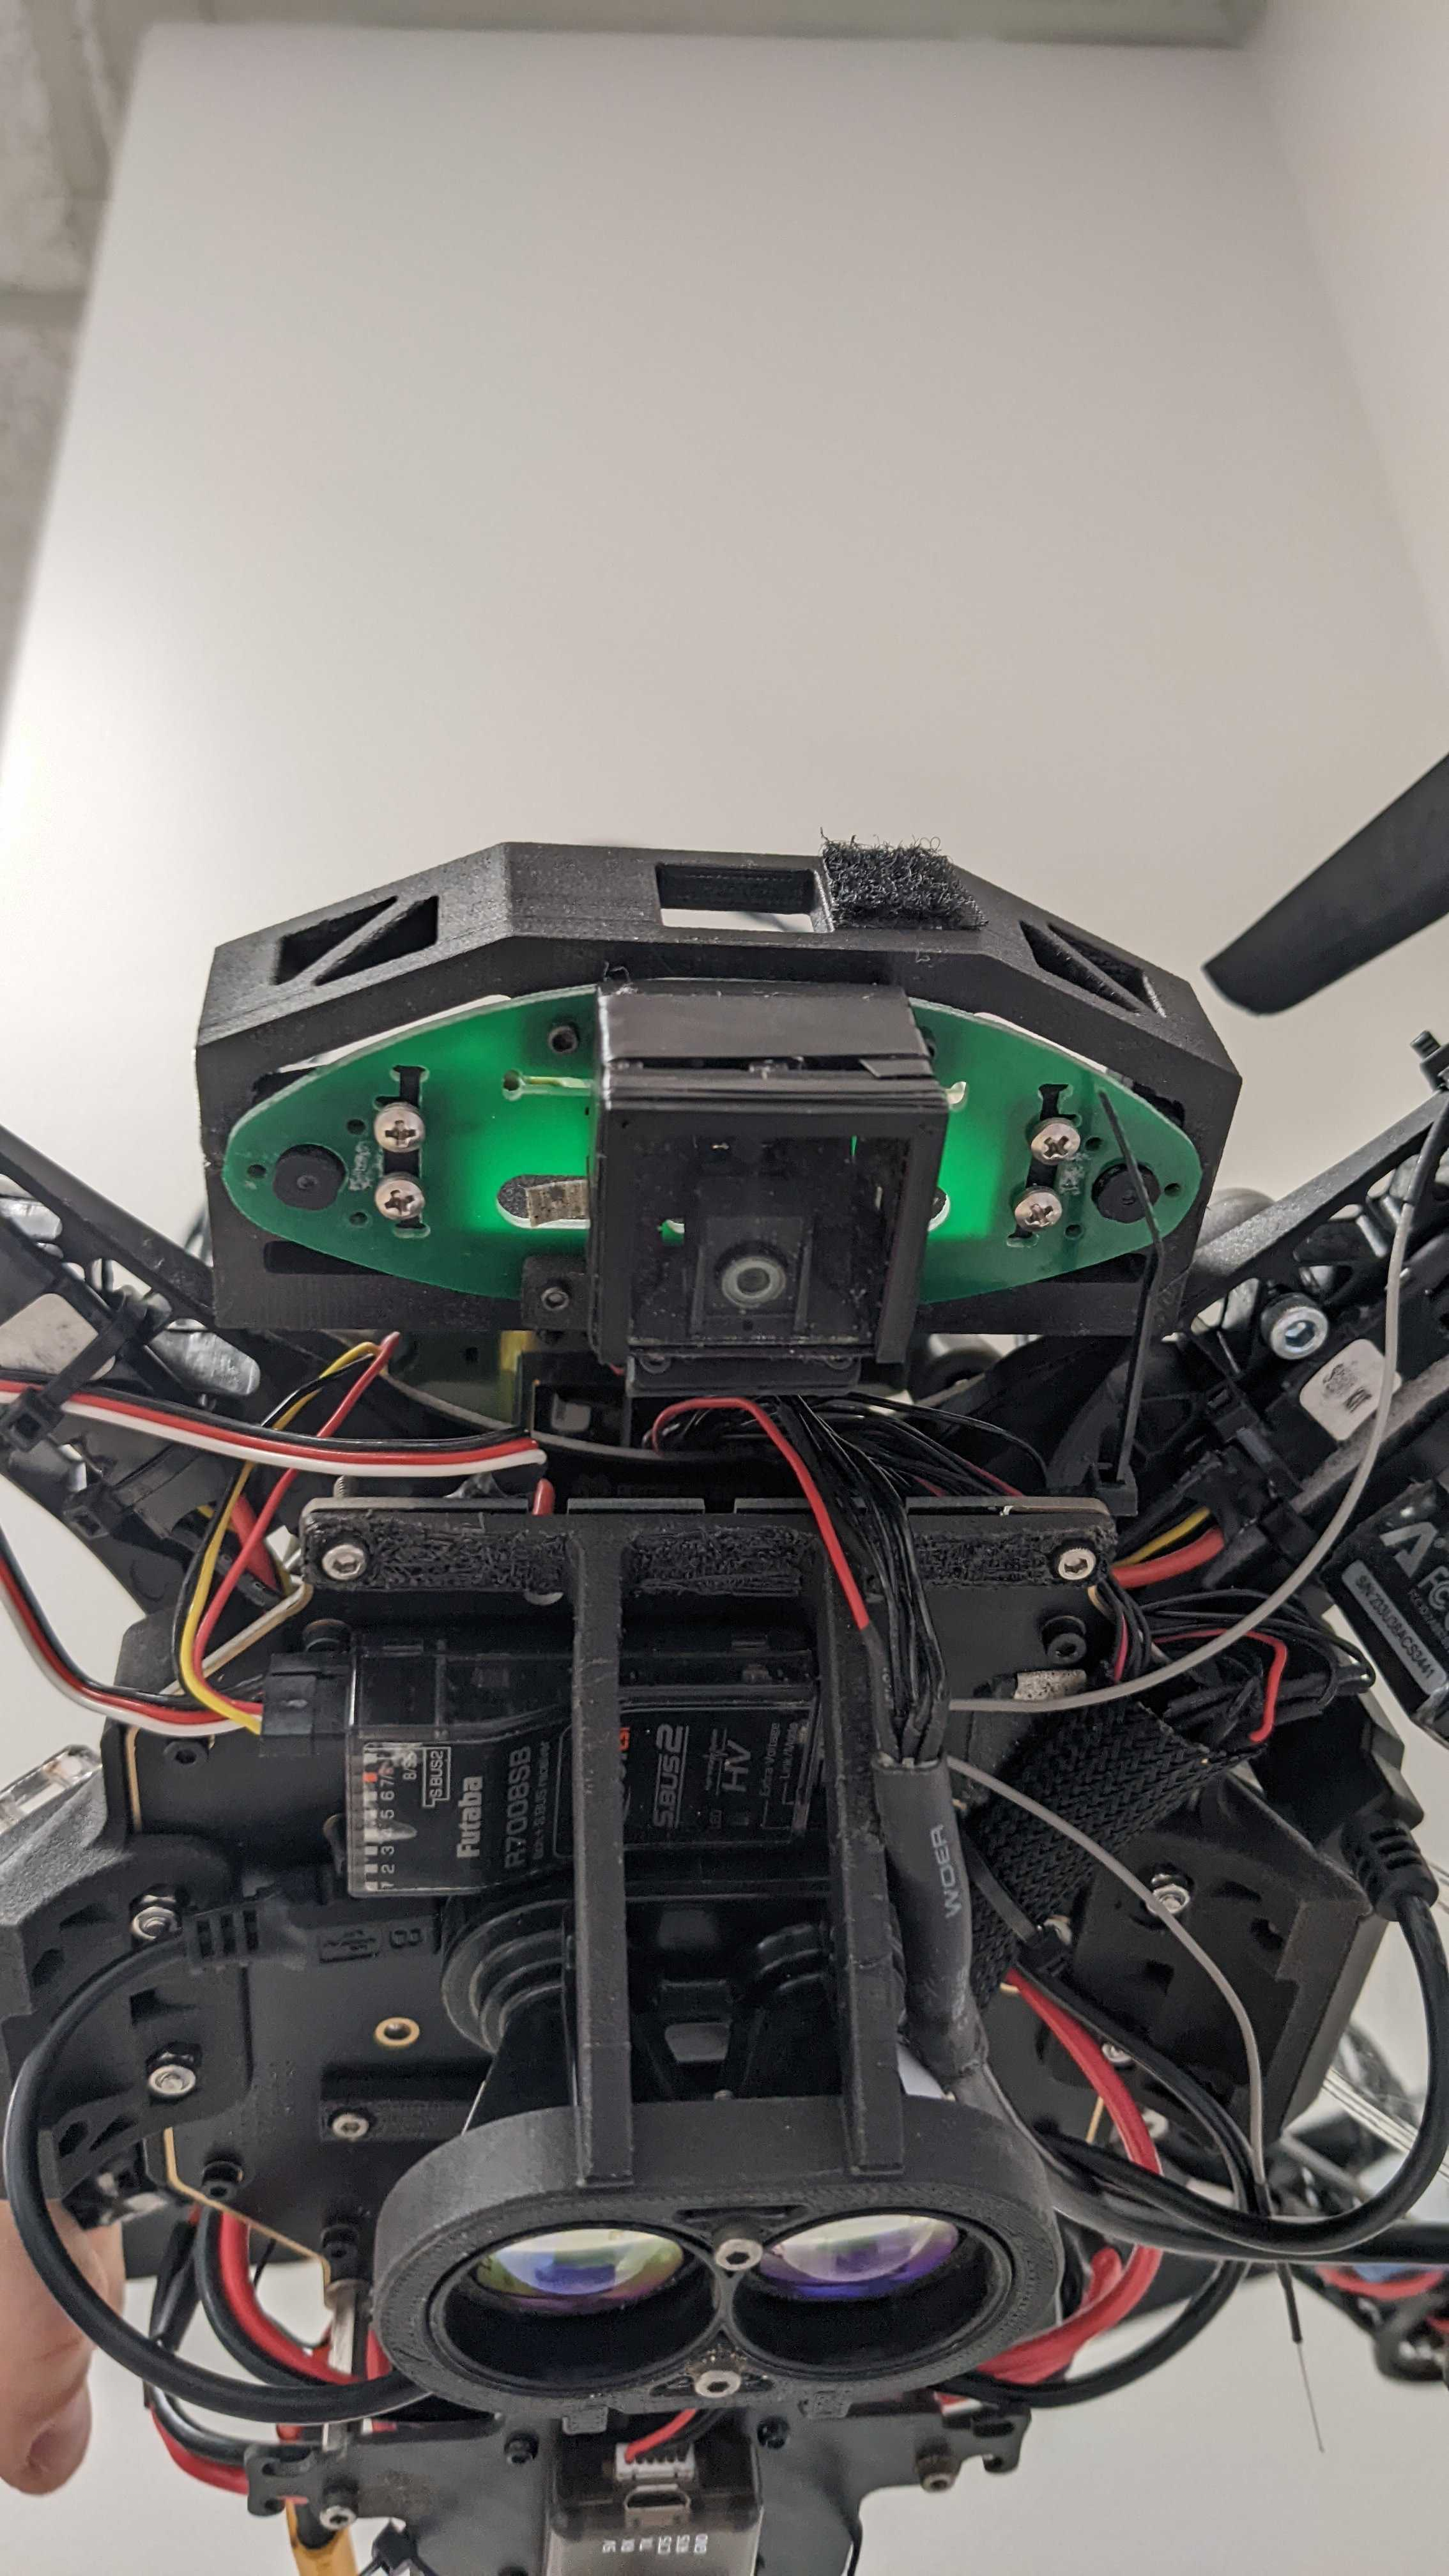
\includegraphics[scale=0.15]{images/appendix/Drone/stereo_cam.jpg}
    \caption{Stereo camera on physical drone}
    \label{fig:appendix_stereo_camera_hardware}
    \end{figure}